\section{Methods}  % TODO good title?
\label{sec:methods}
\subsection{Chandy Misra}
 - src Distributed algorithms by Fokking
 - either write and connec this ro just reference this in the next chapter
\subsection {Fault tolerant Chandy Misra}
  The fault tolerant Chandy Misra version used for our experiments constructs a sink tree in an undirected network under the assumption that a perfect failure detector is present at each node (a detector that does not suspect nodes that haven't actually failed and also will detect each failure eventually). 
  Other than, the original Chandy Misra algorithm this version requires FIFO-channels.
  Furthermore, I assume that the root node cannot fail because otherwise there is no sink tree to construct.
  
  As far as Chandy-Misra is concerned nodes are only interested in crashes of their parents and other ancessor on their path to the root node.
  If a node \co{X} detects a crash of its parent, it sends a \co{REQUEST} message to each neighbour. 
  If a neighbour \co{Y} of \co{X} receives a \co{REQUEST} message, it answers with a \co{DIST d} messages where \co{d} is its own distance. 
  To save message \co{DIST d} is only send if $d < \infty $.
  If \co{Y} happens to be a child of \co{X}, it resets its own \co{dist} and \co{parent} value to $\infty$ respectively $\bot$ and sends a \co{REQUEST} message to all its neighbours.
  
  The requirement for FIFO channels is best understood by a counterexample example on a none FIFO network.
  The network used for this example is shown in \cref{fig:fifoNecessaryNetwork}. 
  Only important messages are mentioned; all other can be assumed to be send and received in any order.
  The Chandy Misra algorithm starts with \co{A} as root node sending \co{DIST 0} messages to \co{B} and \co{C} which on receive consider \co{A} there parent and update their \co{dist} variable.
  They also send \co{DIST} message to their neighbours. 
  When \co{C} and \co{D} receive the \co{DIST} messages from \co{B} respectively \co{C} they consider \co{B} respecitively \co{C} their parents.
  \co{C} sends a \co{DIST TODO} message to \co{D} - lets call it \co{M1}.
  Now \co{B} crashes and when \co{C} detects this, it sends a \co{REQUEST} message towards \co{A} and \co{D} - call the latter \co{M2}.
  If \co{M2} overtakes \co{M1}, \co{D} resets its variabbles and on receive of \co{M1} considers \co{C} its parent which is correct but with an incorrect \co{dist} value of TODO.
  All \co{DIST} messages received by \co{D} from now on have a higher distance value and are dismissed. 
  So the error is never corrected.
  A straightforward fix for this is to use FIFO networks.
  
  SafraFT uses the same FIFO channels as its basic algorithm during the experiment.
  Although, we still claim it does not need this property.
  This claim is straighforward to proof: SafraFT guarantees that at most one message is in any channel at all times because it forwards only a single token and when a backup token is issued, it is send to a different node than the original token and only the first of both tokens is forwarded afterwards.
  Hence, I do not see the use of FIFO channels during the experiment as a problem.
  
  \begin{figure}[h]
  	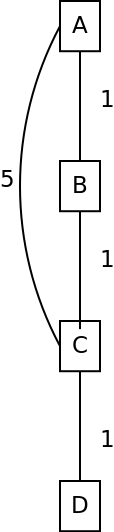
\includegraphics[height=5cm]{figures/FIFO_necessary}
  	\centering
  	\caption{None FIFO network with \co{A} as root to demonstrate necessity of FIFO networks.}	
  	\label{fig:fifoNecessaryNetwork}
  \end{figure}
    
  I argue that this augmented Chandy Misra algorithm constructs correct sink trees in presence of fail-safe failures. 
  Each failure only affects nodes that see themselves as children, grandchildren and so on; that is, it only affects subtrees.
  Because the perfect failure detector guarantees that each node failure will eventually be detected at the children of the failed node, they eventually send \co{REQUEST} message to all their neighbours.
  The neighbours send \co{REQUEST} message to all their neighbours if they receive a \co{REQUEST} message from their parent. 
  Therefore, eventually all nodes in the subtrees of a failing node are reached by \co{REQUEST} message and reset their \co{dist} and \co{parent} values.
  Also all neighbours that receive a \co{REQUEST} message of a node that is not their parent, answer the \co{REQUEST} message with their current \co{dist} value.
  This allows nodes in the affected subtree to rebuild new paths toward the root node.
  These new paths are correct when the answering node is not part of any affected subtree.
  However, if they are part of an affected subtree (e.g. grand children of the crashed nodes), invalid paths are introduced - as these nodes might not be reached by any \co{REQUEST} message and therefore still believe they have a valid path towards root.
  These invalid paths are corrected when the grandchildren are reached by the \co{REQUEST} message of their parent because on receipt they send \co{REQUEST} messages which reset all nodes considering them
  parents. 
  This possible behaviour of introducing invalid paths that are corrected later, might lead to a bad theoretical message complexity but did not hinder the experiments.
  This indicates that this behaviour is not often triggered in praxis.
  
  The presented fault tolerant Chandy Misra algorithm could be improved by relieving the necessity for FIFO-channels, a more formal proof of correctness and a thourough complexity analysis.

  Anyhow, my work suggests that the Chandy Misra version is correct because I run it more than % TODO 
  times and compare the constructed trees to the expected trees which were determined offline. The algorithm yielded the correct sink tree every time.
   
  
 %TODO Provide pseudo code?
 % TODO provide example?
  
\subsection{Fault Simulation}
	I simulate faults by stopping Safra and the basic algorithm on the failing isntance.
	In particular, a crashed node does not send or reacts to tokens or basic messages.
	Faults are triggered before and after interesting events e.g. directly before or after sending a basic message or token. 
	Before every experiment run it is determined at random which node is going to fail, on which event it is going to fail and after how many repetitions of this event e.g. after the 3rd time it forwards a token.
	
	In particular, I selected the following events to trigger a crash if not specified differently the crash is triggered before or after the event:
	\begin{itemize}
	   	\item sending a token (1 to 3 repetitions)
	   	\item sending a backup token (1 to 2 repetitions)
	   	\item before receiving a token (1 to 3 repetitions)
	   	\item sending a basic message (1 to 5 repetitions)
	\end{itemize}
	The range of repetitions is limited to maximize the chance that a node meant to fail actually does so. 
	However, a node that is planned to fail is not guaranteed to do so.
	For example, this leads to runs where 90\% of the nodes should fail but only 88\% do so.
	I verify for every experiment that a reasonable amount of nodes have failed with regard to the planned amount.
	
	Alternatively, to the chosen approach to trigger failures, I considered the more random mechanism of running a thread that kills an instance after a random amount of time.
	One could argue that this would be more realistic.
	However, I believe this kind of a approach leads to less interesting failures because the vast majority of these failure would occure during idle time. 
	Furthermore, most failures between internal events are observed as exactly the same on all other nodes. 
	For example, other nodes cannot observe if a failure happened before an internal variable changed or after. 
	In fact, they can only observe a difference when the failure happens after or before sending a message to them.
	Hence, I have chosen a fault mechanism that focusses on these distinguishable scenarios.
	As one might notices, the failure points are chosen to give raise to many different situations for our Safra versio to deal with. 
	I deliberately decided against chosing special failure points with regard to the basic algorithm because this would be lead to less focussed testing of the fault tolerance of Safra.
	
\subsection{Fault Detection}
Our Safra version assumes the presence of a perfect fault detector.
This kind of fault detection is easy to implement and integrate with the system e.g.
\cite{fokkink:2018} on page 113 describes a straightforward implementation.

% TODO do I want a second reference e.g. a paper that shows an implementation
As building a perfect fault detector is a well known and solved problem, but nonetheless time consuming, I decided to avoid implementing one.
For this experiment fault detection is simulated by sending \co{CRASH} messages from crashing nodes to its neighbours. 
This leads to a realistic fault detection model because these messages are sent asynchronlously through the same channels as all other messages. 
Hence, closely imitating a perfect failure detector based on heartbeats. 
In particular, a fault is detected \textit{eventually after} it happened as with every failure detector.
\co{CRASH} messages are not broadcasted to all nodes because IBIS (the message passing library I used) does not provide broadcasting.

After running the experiments, I noticed a limitation due to my fault detection mechanism:
configurations in which a message is received from a node after its crash was detected, do not arise because I use FIFO channels for all messages.  %TODO connect to the argumentation for these channels.
This could be easily fixed by using dedicated channels for crash messages - in IBIS this would manifest in dedicated "crash message" ports on each node.
Then receiving crash messages would be out-of-band with regular message and the order of receiption would depend on sending time, the Linux scheduler and IBIS implementation details.
The last two points are the reason why I decided against that approach at first.

% TODO fix and run a few goes to provide evidence this does not matter
  

\subsection{Offline Analysis}
 % TODO is that more in Results on defintion from token after termination.
 We measure tokens before and after termination
 - define 
 - tokens after termination
 - actual termination (not real point of time for termination)
 defintion:
 1. No messages in the channels
 2. All nodes are passive
 3. Termination is postponed until all nodes that need to take action on any fault, detected the regarding fault. Only nodes which parent node fails need to take action and this might trigger further events in any other node.
 - detected termination
 
 - needs means of determining termination independent and closer to actual termination than Safra
 - by logging token count, time spent events, active status change, message counter change (mean to determine no messages in the cahnnel) and parent crash detected
 - based on this detecting actual termination
 - by logging token count, time spent events. Dividing in before and after termination.
 
 - Also using it for verification  see \cref{verifaction}

\subsection{Environment}
\subsubsection{IBIS}
  IBIS is a Java-based platform for distributed computing developed by researchers of the Vrije Universiteit Amsterdam. 
  Its suppart IPL is used as the message passing library for this project. 
  I use version 2.3.1 which can be found on GitHub: \href{https://github.com/JungleComputing/ipl/releases/tag/v2.3.1}{https://github.com/JungleComputing/ipl/releases/tag/v2.3.1}.
  
  Communication channels in IPL are backed by TCP and provide asynchronous messaging.
  For this experiments, I also used IPL's ability to guarantee FIFO channels.
\subsubsection{DAS 4}
  The experiment was conducted on the part of DAS-4 that belongs to the Vrije Universiteit Amsterdam. 
  The nodes use primarily SuperMicro 2U-twins with Intel E5620 CPUs and a Linux CentOS build with the kernel version 3.10.0-693.17.1.el7.x86\_6.
  For communication 1Gbit/s Lan was used.
  At time of the experiments the VU had 41 nodes with 8 cores per node.
  Therefore, multiple instances were run on each physical node.
  This is possible because Safra and Chandy Misra are both communication heavy with rather low processing and memory requirements.
  % TODO AFK
 
\subsubsection{Network Topology}
  The basic algorithm I use take a network topology to work on as input. 
  They require an undirected network.
  To generate more interesting runs I use weighted networks.
  
  Our Safra version needs an undirected ring. 
  For simplicity in my setup this ring is part of the network the basic algorithms run on. 
  That means no matter which network topology the basic nodes are running on, there is always an undirected ring available in the network topology.
  
  All networks for the experiments are generated by choosing randomly between 1 and 5 neighbours for each node and assigning a random, unique weight between 1 and 50000 to each channel.
  
  After this channels with the heavyweight of 400000 are added between the root and some nodes to ensure the network stays connected when nodes fail.
  For this I calculate the expected network with knowledge of the predetermined failing nodes and add more connections between probably disconnected nodes and the root.
  These channels are so heavyweight to avoid using them over `regular' channels which might create highly similiar topologies with a lot of nodes connected to the root directly.
  
  At last, channels are added to form an undirected ring in which each channel has the weight of 100000. 
  Again the weight is chosen to avoid `overusing' the ring channels for the trees built.
  
  For the experiments, I am not interested in the relationship between network topology and our metrics because this kind of analysis seems to detailed to show correctness of our Safra version or to compare
  our Safra version with the traditional Safra version.
  Therefore, the exact network topology is not recorded. 
  Anyhow, I output the depth of resulting trees and the nodes per level for runs up to 500 nodes.
  These metrics are recorded in the final result to allow for quality checks and ensure the experiments were not run on trivial networks.
  Generating this statistics for runs with over 500 nodes turned out to be time consuming.
  Hence, I decided not to generate them.
  However, if the network topology leads to none trivial, deep trees with 500 nodes and less, it seems highly unlikely that it would not with even more nodes.
  Furhtermore, I verified that the topology with more than 500 nodes generates still interesting cases by spot sample.
  